\documentclass[11pt,spanish,a4paper]{article}
% Versión 1er cuat 2015 Víctor Bettachini < bettachini@df.uba.ar >

\usepackage{babel}
\addto\shorthandsspanish{\spanishdeactivate{~<>}}
\usepackage[utf8]{inputenc}
\usepackage{float}
\usepackage{units}
\usepackage{siunitx}
\usepackage{amsmath}
\usepackage{amstext}
\usepackage{amssymb}
\usepackage{graphicx}
\graphicspath{ {./graphs_armonico/} {../}}

\voffset-3.5cm
\hoffset-3cm
\setlength{\textwidth}{17.5cm}
\setlength{\textheight}{27cm}

\usepackage{lastpage}
\usepackage{fancyhdr}
\pagestyle{fancyplain}
\fancyhead{}
\fancyfoot{{\tiny \textcopyright Departamento de Física, FCEyN, UBA}}
\fancyfoot[C]{{\tiny Actualizado al \today}}
\fancyfoot[RO, LE]{Pág. \thepage/\pageref{LastPage}}
\renewcommand{\headrulewidth}{0pt}
\renewcommand{\footrulewidth}{0pt}


\begin{document}
\begin{center}
  \textbf{Física 2} (Físicos) \hfill \textcopyright {\tt DF, FCEyN, UBA}\\
  %\textsc{\large Física 2 (Físicos)} - Prof. Hernán Grecco - 1"er cuat. 2015\\
  \textsc{\large Guía 1:} Oscilador armónico
\end{center}
\centering
\emph{Nota general: en todos los problemas analice a priori qué puede predecir sin
	hacer cálculos y analice a posteriori qué podría haber predicho sin hacer
cálculos.}


\begin{enumerate}


\item Escriba la ecuación del péndulo para las coordenadas \(x\), \(z\) y \(\varphi\).
	Escriba la energía potencial y cinética en dichas coordenadas.
	Discuta cuáles elecciones son convenientes y cuáles no.
	\begin{figure}[h]
		\centering{}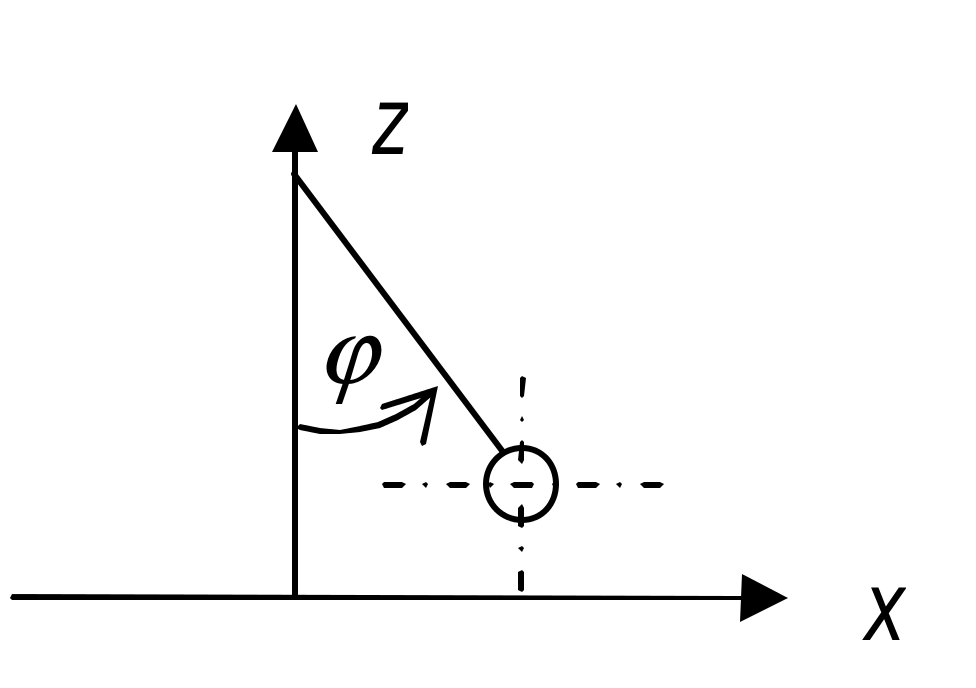
\includegraphics[width=0.35\textwidth]{guia1_e1}
	\end{figure}


\item Resuelva el péndulo en pequeñas oscilaciones tomando como coordenada el
	ángulo \(\varphi\) entre el hilo y la horizontal (techo).


\item Demuestre que si \(\Psi\) es una solución matemática compleja de la ecuación del oscilador armónico, su parte real también es solución.


\item Escriba y resuelva las ecuaciones de movimiento para los siguientes sistemas:
	\begin{enumerate}
		\item Péndulo de longitud \(l\) en presencia de un campo gravitatorio de constante \(g\).
			Discuta todas las aproximaciones que realiza.
			Demuestre que sin dichas aproximaciones la superposición lineal de dos soluciones no es solución (el sistema no es lineal).

		\item Oscilaciones longitudinales de una masa \(m\) sujeta a dos paredes mediante dos resortes iguales de constante \(k\) (ver figura).%; para los dos casos:
		% \begin{enumerate}
		% 	\item longitud natural del resorte $l_{0}$ $(l_{0}<l)$, y
		% 	\item ``slinky'' $(l_{0}=0)$.
		% \end{enumerate}

		\item Oscilaciones transversales del sistema del punto anterior, en los siguientes casos límite en que el resorte:
			\begin{enumerate}
				\item está poco estirado, es decir \(l\) no mucho mayor que su longitud natural \(l_0\) (sin fuerza)
				\item es muy elongable (caso llamado ``slinky''), de forma que puede considerarse que \(l_{0}\simeq0\)
			\end{enumerate}

	% \item Oscilaciones transversales del sistema del punto anterior, discutiendo las diferencias entre los casos 1) y 2), y analizando cuidadosamente las aproximaciones que realiza.
			Analice \textbf{cuidadosamente} las aproximaciones requeridas en el primer caso.
			Describa la diferencia entre considerar que los resortes están tensionados en la posición de equilibrio (\(l_{0}<l\)) o que están relajados en dicha posición (\(l_{0}=l\)).
			Compare las frecuencias de los modos longitudinales y transversales.
			% En el caso 1) analice la diferencia entre considerar que los resortes están tensionados en la posición de equilibrio $(l_{0}<l)$ o que están relajados en dicha posición $(l_{0}=l)$.
			\begin{figure}[h]
				\centering{}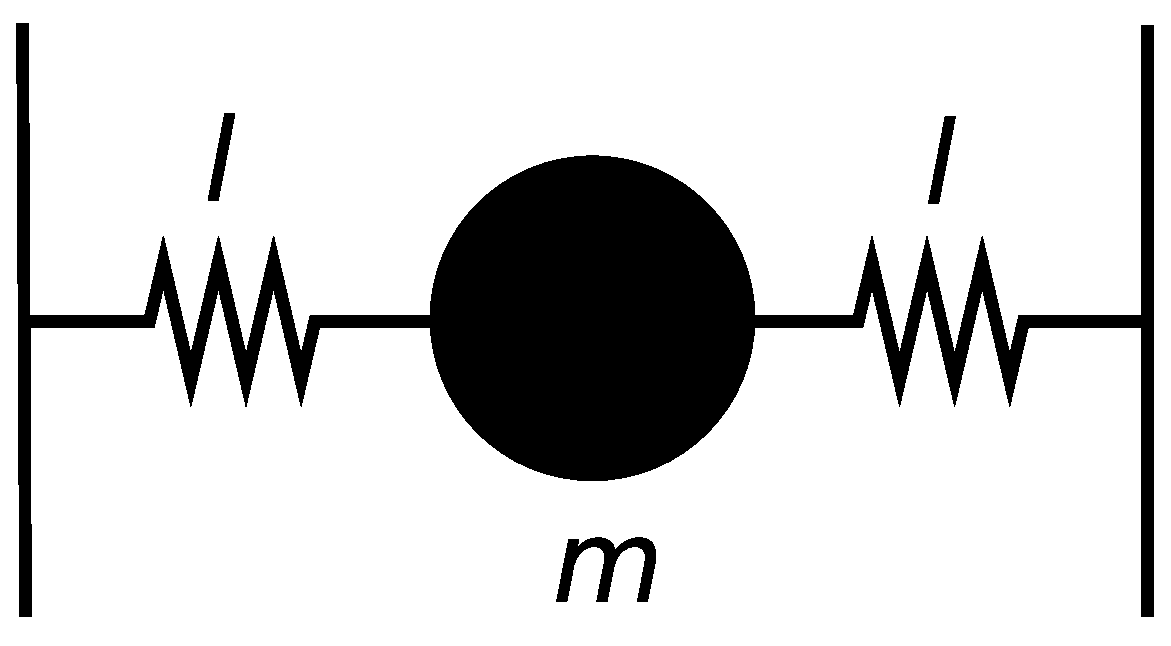
\includegraphics[clip,scale=0.25]{ej1-1}
			\end{figure}
	\end{enumerate}


\item Resuelva el resorte vertical con un peso colgado usando como cero de coordenadas la del resorte en reposo sin peso.
	Escriba la energía potencial (gravitatoria más elástica) y encuentre la posición de equilibrio.
	Analice la curvatura de dicho potencial.
	Al oscilar, ¿la energía potencial es solo la del resorte o también oscila la potencial gravitatoria?


\item Calcule la tensión del hilo en función del ángulo para un péndulo en pequeñas
	oscilaciones. Discuta la validez de la hipótesis de longitud de hilo constante.


\item Para un péndulo con fuerza de disipación proporcional a la velocidad calcule el
	trabajo que realiza la fuerza de rozamiento y compárelo con la pérdida de energía.


\item Verifique que si \(\Psi_1\) y \(\Psi_2\) son soluciones de la ecuación del oscilador armónico libre, cualquier combinación lineal \(\Psi= A_1 \Psi_1+ A_2 \Psi_2 \) también es solución.
	Muestre que esto también vale si la fuerza disipativa es proporcional a la velocidad.
	¿Vale si es un rozamiento constante?


\item Se tiene un péndulo que oscila con una disipación tal que su amplitud se reduce un 10\% cada 10 oscilaciones.
	¿Con que precisión deberíamos determinar su longitud para notar el corrimiento en su frecuencia debido al rozamiento?


\item Resuelva un oscilador armónico libre al que se le agrega una fuerza de rozamiento constante.
	Sugerencia: resuelva cada media oscilación agregando la fuerza que cambia la
	posición de equilibrio.
	Calcule el movimiento cada medio ciclo.
	Evalúe como cambia la amplitud cada medio ciclo.
	Calcule como es esa amplitud máxima en función del número de oscilación y compárela con una fuerza disipativa proporcional a la velocidad.


\item
	\begin{enumerate}
		\item Resuelva de manera completa el oscilador forzado excitado en el pico de resonancia (\(\omega =\omega_0 \)) con la condición inicial de estar en reposo en su posición de equilibrio.

	\item Simplifique la expresión para el caso en que \(\gamma \ll \omega_0\) y grafíquela para poner en evidencia como el sistema tiende a su solución estacionaria.
	\end{enumerate}

\end{enumerate}

\end{document}
